\section{Comparación con otros métodos de diagnóstico}

\subsection{Resonancia Magnética vs. Rayos X}

La resonancia magnética (RM) y los rayos X son técnicas de diagnóstico por imagen que se basan en principios físicos completamente distintos. 
Los rayos X emplean radiación electromagnética ionizante con longitudes de onda del orden de $10^{-10}\,\text{m}$, que interacciona con los electrones de los tejidos. 
La atenuación de la intensidad sigue la ley de Beer–Lambert:

\begin{equation}
I = I_0 e^{-\mu x}
\end{equation}

donde $I_0$ es la intensidad inicial, $I$ la intensidad transmitida, $\mu$ el coeficiente de atenuación y $x$ el espesor del material. 
Esto implica que los tejidos más densos, como los huesos, absorben más radiación, generando mayor contraste en la imagen.

En cambio, la RM se fundamenta en la resonancia de los núcleos de hidrógeno sometidos a un campo magnético intenso $B_0$. 
La frecuencia de precesión de estos núcleos está dada por la \textbf{ecuación de Larmor}:

\begin{equation}
\omega_0 = \gamma B_0
\end{equation}

donde $\omega_0$ es la frecuencia angular de resonancia y $\gamma$ la constante giromagnética del protón ($\gamma/2\pi \approx 42.58\,\text{MHz/T}$). 
A diferencia de los rayos X, la RM no utiliza radiación ionizante, lo que reduce los riesgos biológicos. 
Sin embargo, su tiempo de adquisición es mayor y el equipo considerablemente más costoso.

\begin{figure}[h!]
    \centering
    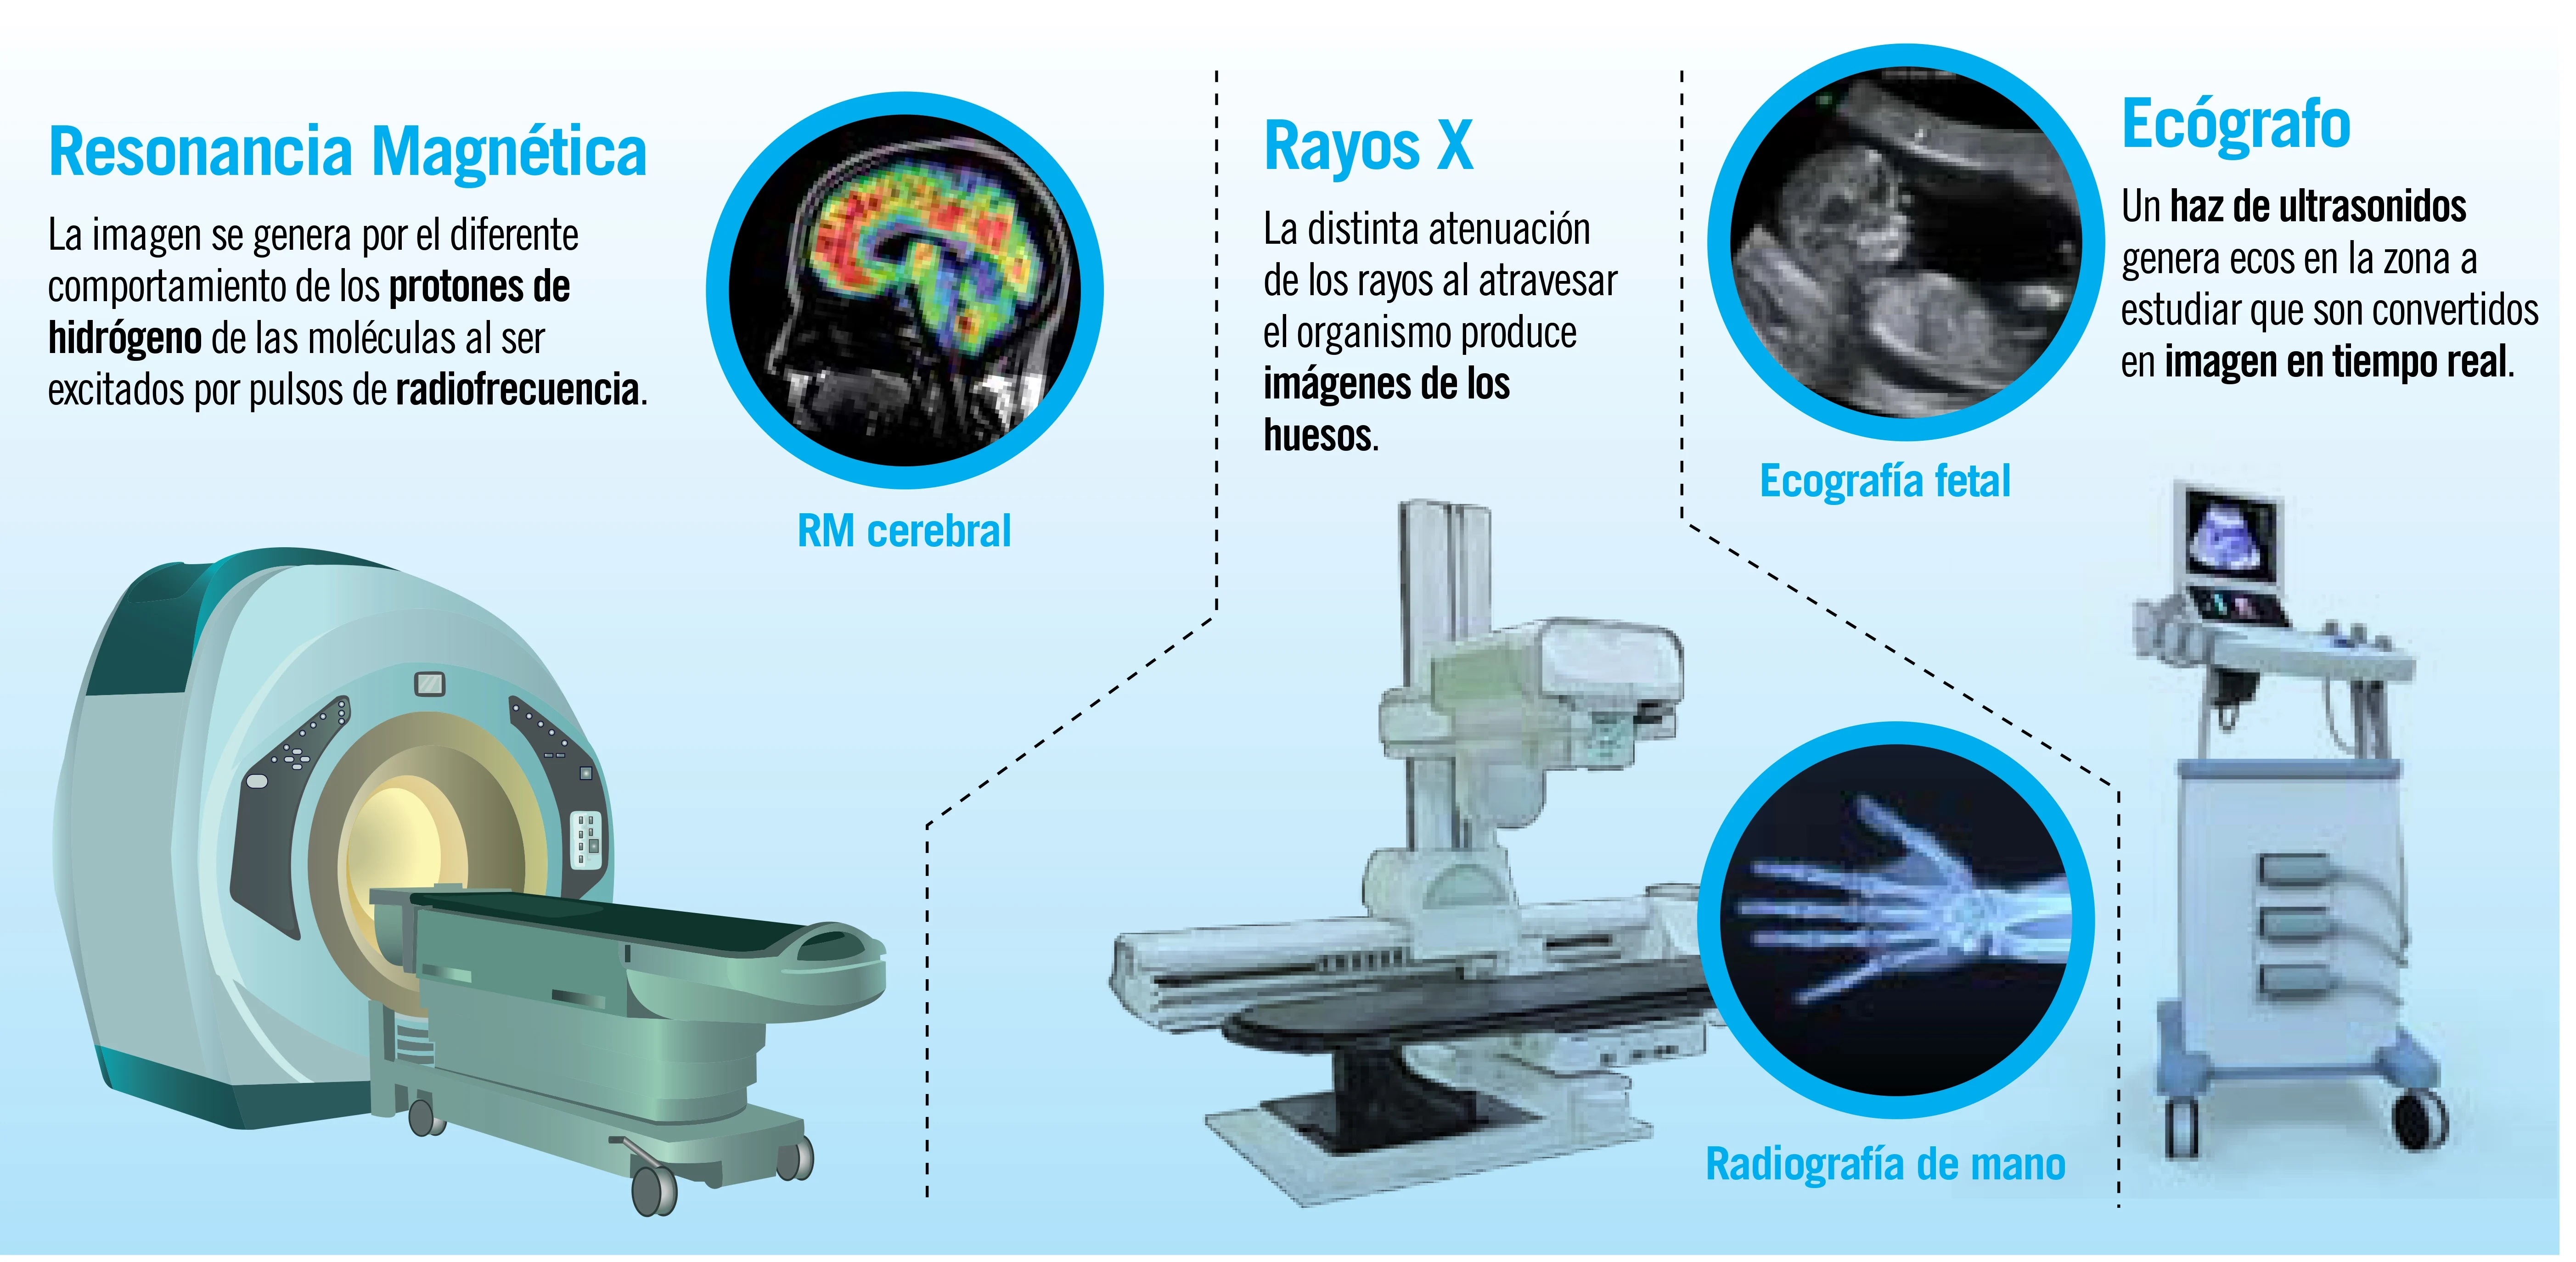
\includegraphics[width=0.7\textwidth]{img/rayosx_vs_rm.png}
    \caption{Comparación esquemática entre rayos X (izquierda) y resonancia magnética (derecha).}
\end{figure}

\subsection{Resonancia Magnética vs. Tomografía Computarizada (TC)}

La tomografía computarizada (TC) también utiliza rayos X, pero en múltiples proyecciones que son reconstruidas mediante algoritmos computacionales, obteniendo imágenes tridimensionales. 
La intensidad detectada en cada ángulo se relaciona con la densidad electrónica del material. 
El proceso de reconstrucción se basa en la \textbf{transformada de Radon} $R[f(x,y)]$:

\begin{equation}
R[f(x,y)](\theta, s) = \int_{-\infty}^{\infty} f(s\cos\theta - t\sin\theta, s\sin\theta + t\cos\theta)\, dt
\end{equation}

y su inversa permite reconstruir la imagen interna del cuerpo.

Por su parte, la RM genera imágenes a partir de la respuesta de relajación de los espines nucleares tras aplicar pulsos de radiofrecuencia. 
Los dos parámetros fundamentales son:

\[
T_1: \text{tiempo de relajación longitudinal}, \quad 
T_2: \text{tiempo de relajación transversal.}
\]

Estos definen el contraste de la imagen según las expresiones:

\begin{align}
M_z(t) &= M_0 \left(1 - e^{-t/T_1}\right), \\
M_{xy}(t) &= M_0 e^{-t/T_2}
\end{align}

donde $M_z$ representa la magnetización en la dirección del campo principal y $M_{xy}$ la componente transversal. 
Mientras la TC resalta diferencias de densidad, la RM distingue variaciones en la composición química y molecular de los tejidos, como el contenido de agua y grasa.

\begin{figure}[h!]
    \centering
    \includegraphics[width=0.7\textwidth]{img/tc_vs_rm.png}
    \caption{Comparación esquemática entre TC y RM.}
\end{figure}

\subsection{Resonancia Magnética vs. Ecografía}

La ecografía utiliza ondas mecánicas (ultrasonido) con frecuencias entre 1 y 15 MHz. 
El principio físico se basa en la reflexión parcial de ondas acústicas en las interfaces de tejidos con distinta impedancia acústica $Z = \rho c$, donde $\rho$ es la densidad y $c$ la velocidad del sonido.

El coeficiente de reflexión se expresa como:

\begin{equation}
R = \left( \frac{Z_2 - Z_1}{Z_2 + Z_1} \right)^2
\end{equation}

Mientras que la RM emplea campos magnéticos y radiofrecuencia, sin involucrar propagación mecánica. 
La ecografía es más adecuada para estudios dinámicos y superficiales (por ejemplo, monitoreo fetal o estructuras musculares), mientras que la RM ofrece mayor resolución en tejidos blandos profundos y análisis espectroscópico.

En términos energéticos, la RM opera en el rango de microondas ($10^7$–$10^8\,\text{Hz}$), con energías asociadas:

\begin{equation}
E = \hbar \omega_0 = \hbar \gamma B_0
\end{equation}

mucho menores que las de los rayos X ($E \approx 10^3$–$10^5\,\text{eV}$), lo que explica su inocuidad radiobiológica.
